\normalsize
\begin{flushleft}
    \section{Technical Design}

    \subsection{Programming Language Selection and Libraries Used}

    I selected C# as my programming language for several reasons. Currently, it is the language that I am most familiar with. In addition, I conducted research on which languages are best for fast processing, and found that C, C++, and C# are among the top contenders. Considering my skill set and the importance of speed in this situation, I concluded that C# would be a good fit. Furthermore the object orientated nature of the language means that I will be able to separate the front end and the back end processing into separate bll files keeping the code clean and easily maintainable.\\ 
    \bk
    Find below a list of all libraries I used: \\
    
    \subsubsection{Linq}
    In order to manipulate lists and create the data structures that I need I will need to use some Linq methods. During the prototyping stage I found that using some Linq methods such as the Select statement allowed the program to be easier to read and make logical sense. As well as this there have been optimisations made in the iterative Linq methods which will make my program faster. Similar to some of the following libraries this is a Microsoft Library which is open source.
    \\ \bk


    \subsubsection{Bitmap}
    In order for my program to function a required part of it is that it is able to take an image as an input. In native C# there is no set way to do this. Therefore I needed to use the Microsoft System.Drawing Namespace. This namespace provides access to GDI+ basic graphics functionality. This does limit this project as is to only working on Windows since the library requires access to the GDI+ native library which is only on windows services. \\
    
    The only part of this library I will be using is the Bitmap class. This will allow me to accept all types of images without the need of parsing them myself since this is not the aim of my project. 
    \\ \bk

    \subsubsection{Windows Forms}
    In order to complete my objectives my program will need to be easy to use and any user with some degree of technical competency should be able to use it. In order to achieve this objective I though that instead of using some form of console input in order to get a starting and an end location, that it would be better to use some form of GUI. In order to do this I will use Windows Forms. This will allow me to make a simple GUI which will allow the end user to interact with the user and easily understand. \\ 

    The things which I will end up using the windows forms are the map traversal, allowing the user to select a start and an end node with a click instead of having to enter a coordinate. As well as this I will also use forms to show the user the stages of, for example, the canny edge detection.
    \\ \bk

    \subsection{High Level Overview}
    The general purpose of my project is to allow a user to take a map and input it into my program, then subsequently convert it into a routable map. \\ \bk
    
    In order to achieve this goal my program will first take an input, the users map. It will then take this map and convert it into an machine readable format, a Bitmap. Canny edge detection will then be performed on it causing the edges and the surroundings of the paths on the image to be found. Using these edges a filling algorithm will fill the spaces encapsulated by the lines. Finally these filled spaces will be used to convert the whole image to a graph which can then be traversed using graph traversal algorithms such as A* or Dijkstra's algorithm. \\ \bk

    \begin{figure}[H]
        \centering
        \subfloat[\centering High Level Overview Of Program]{{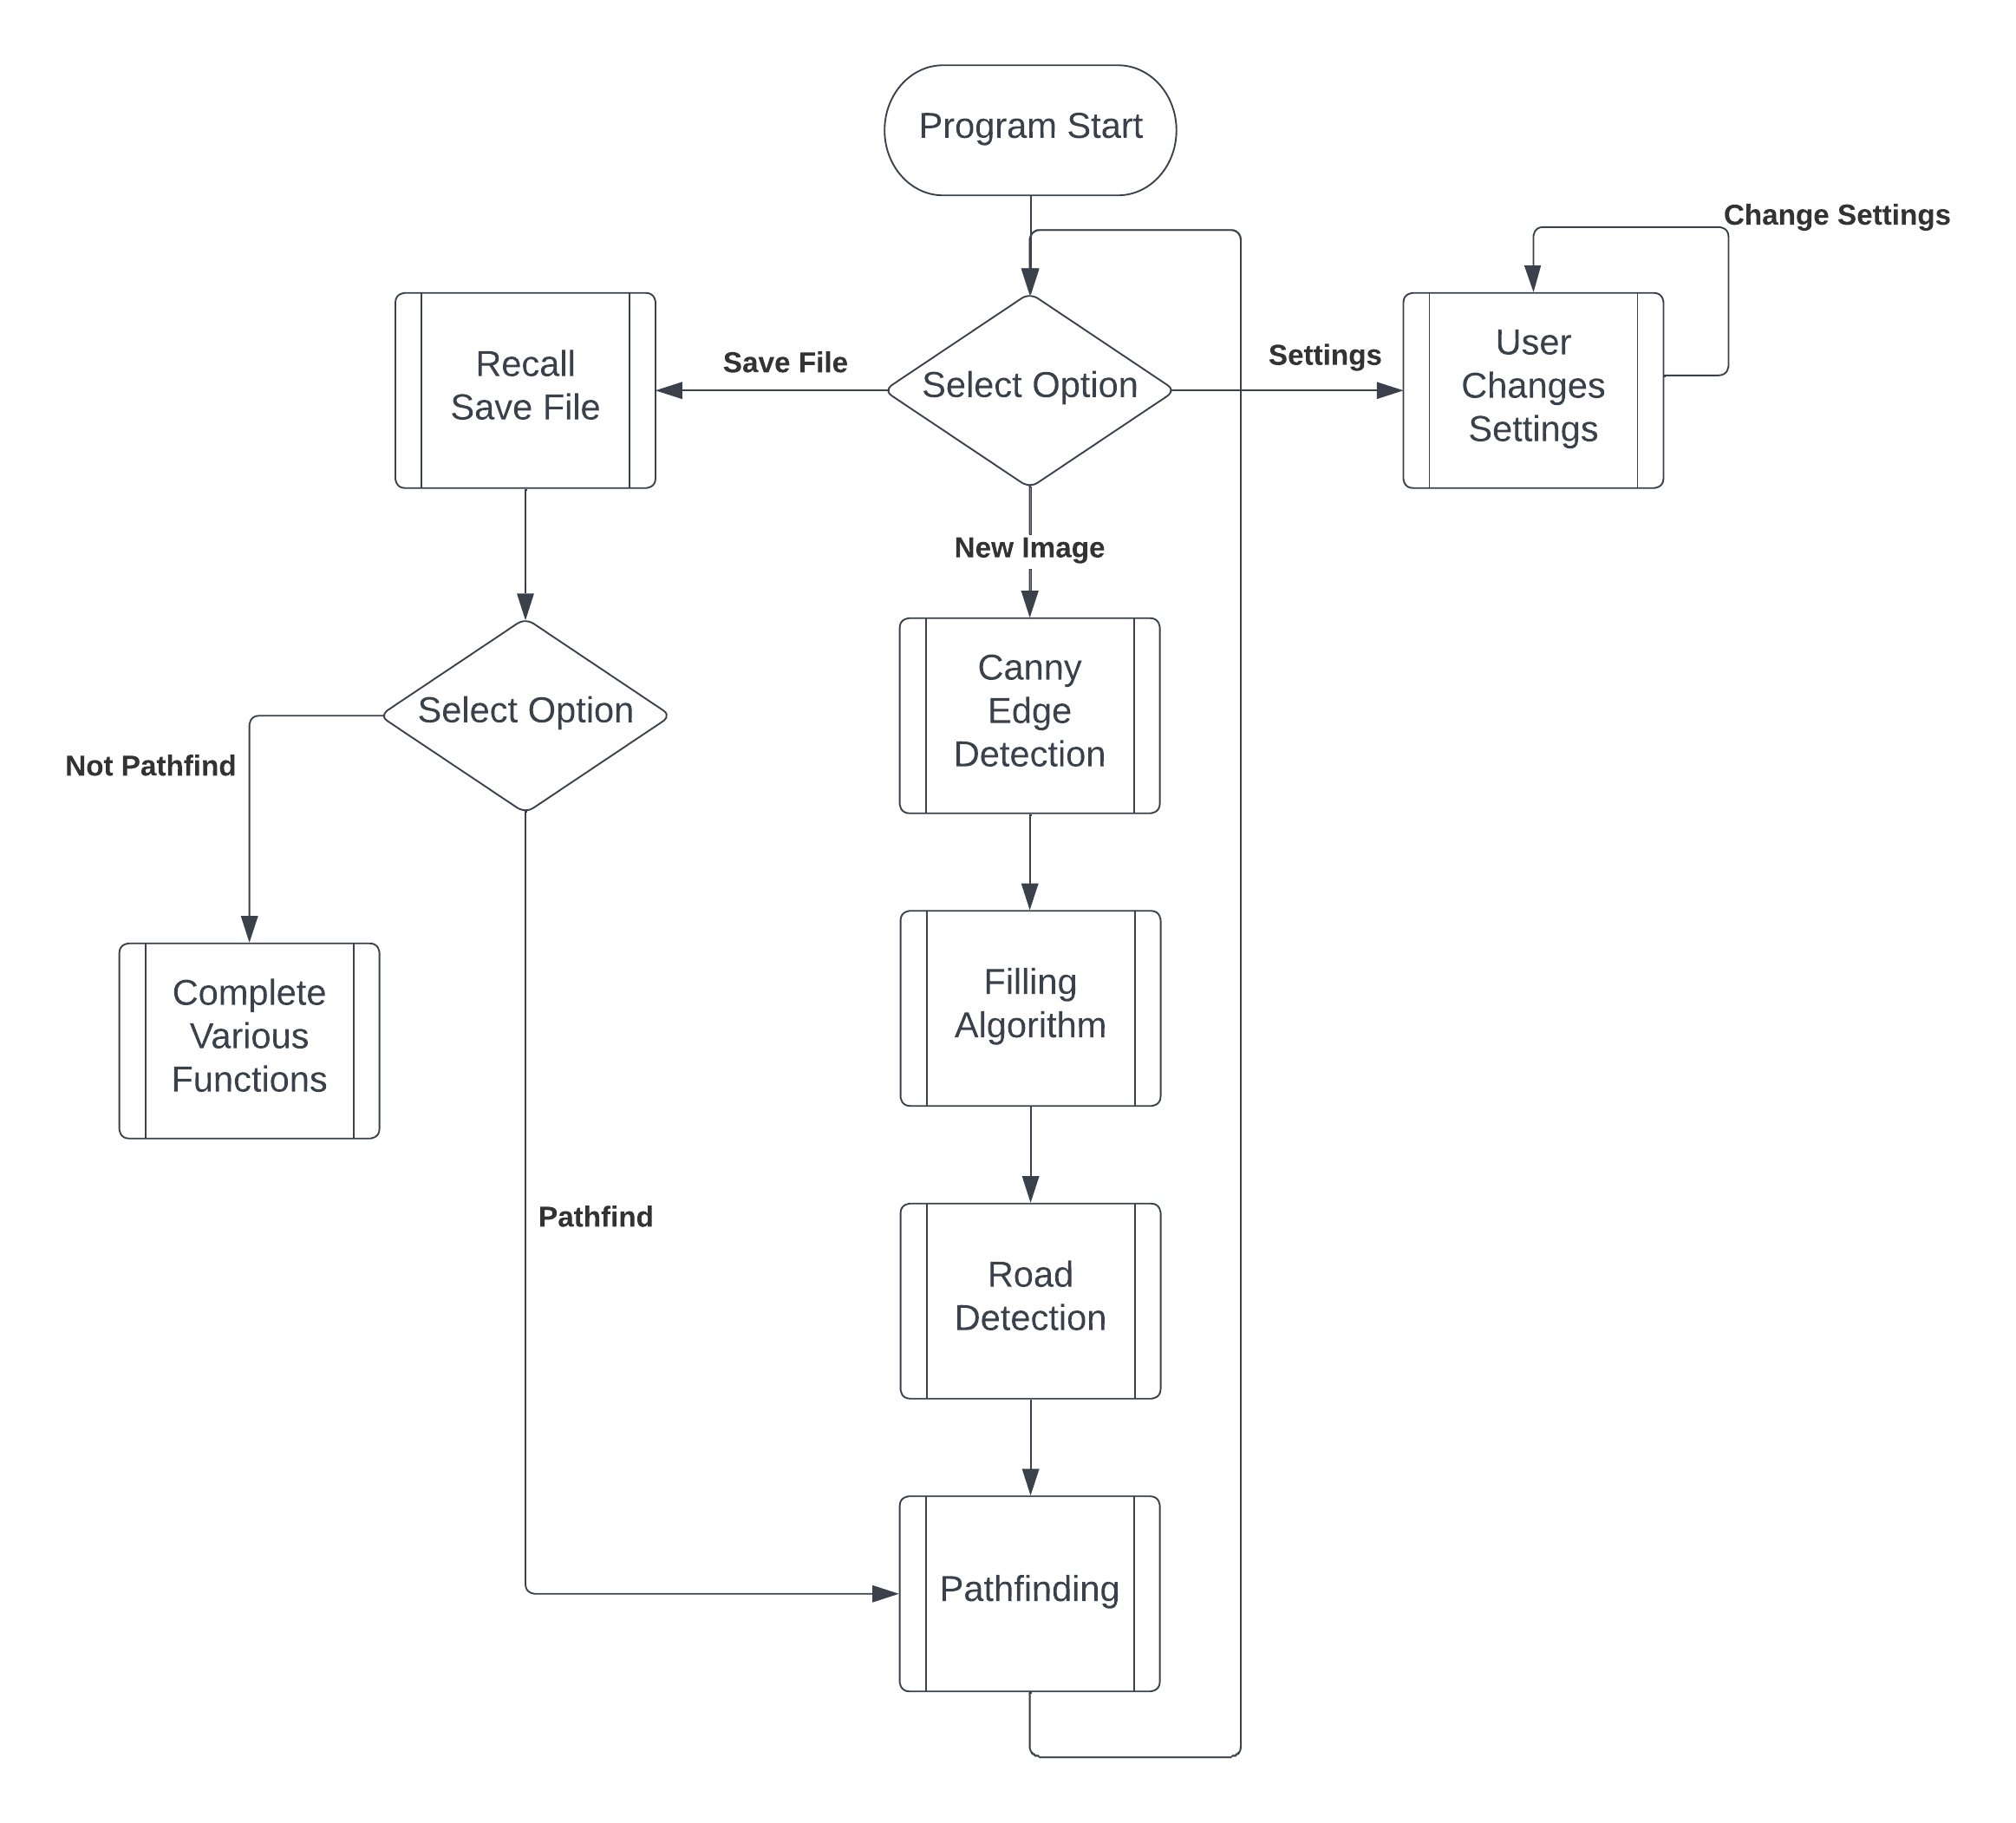
\includegraphics[width=17.2cm]{images/HighLevelOverview.png}}}
    \end{figure}

    The version of Edge Detection I will be using as previously stated will be Canny Edge Detection, this is as opposed to Sobel Edge Detection. The main version of filling I will be using is flood fill due to it simple nature to implement ad due to the fact that it does not take much memory and can be made recursive so it performs well. The final main algorithm I will need to use is image kernels and convolution, this will allow me to manipulate the inputted image.

    \subsubsection{Backend Library}
    For my project to ensure that I conform to the OOP principle of encapsulate what varies. I will accomplish this through the use of classes and encapsulation. Furthermore I have also made the decision to split up my solution into two separate projects, this means that my program will produce two files in order to run, one of these will be the DLL for the backend library and the other will be the executable for the front end. \\ \bk

    Contained within this backend section of my program will be contained the edge detection, road detection, complex data types and graph traversal algorithms as well as various utilities that are frequently used throughout the program. \\ \bk

    One of the main features of the backend library are the custom structures that have been created in order to allow for easier processing of data. Find below the image of the structure class layout and the classes which link within.

    \begin{figure}[H]
        \centering
        \subfloat[\centering Overview of Backend Structures]{{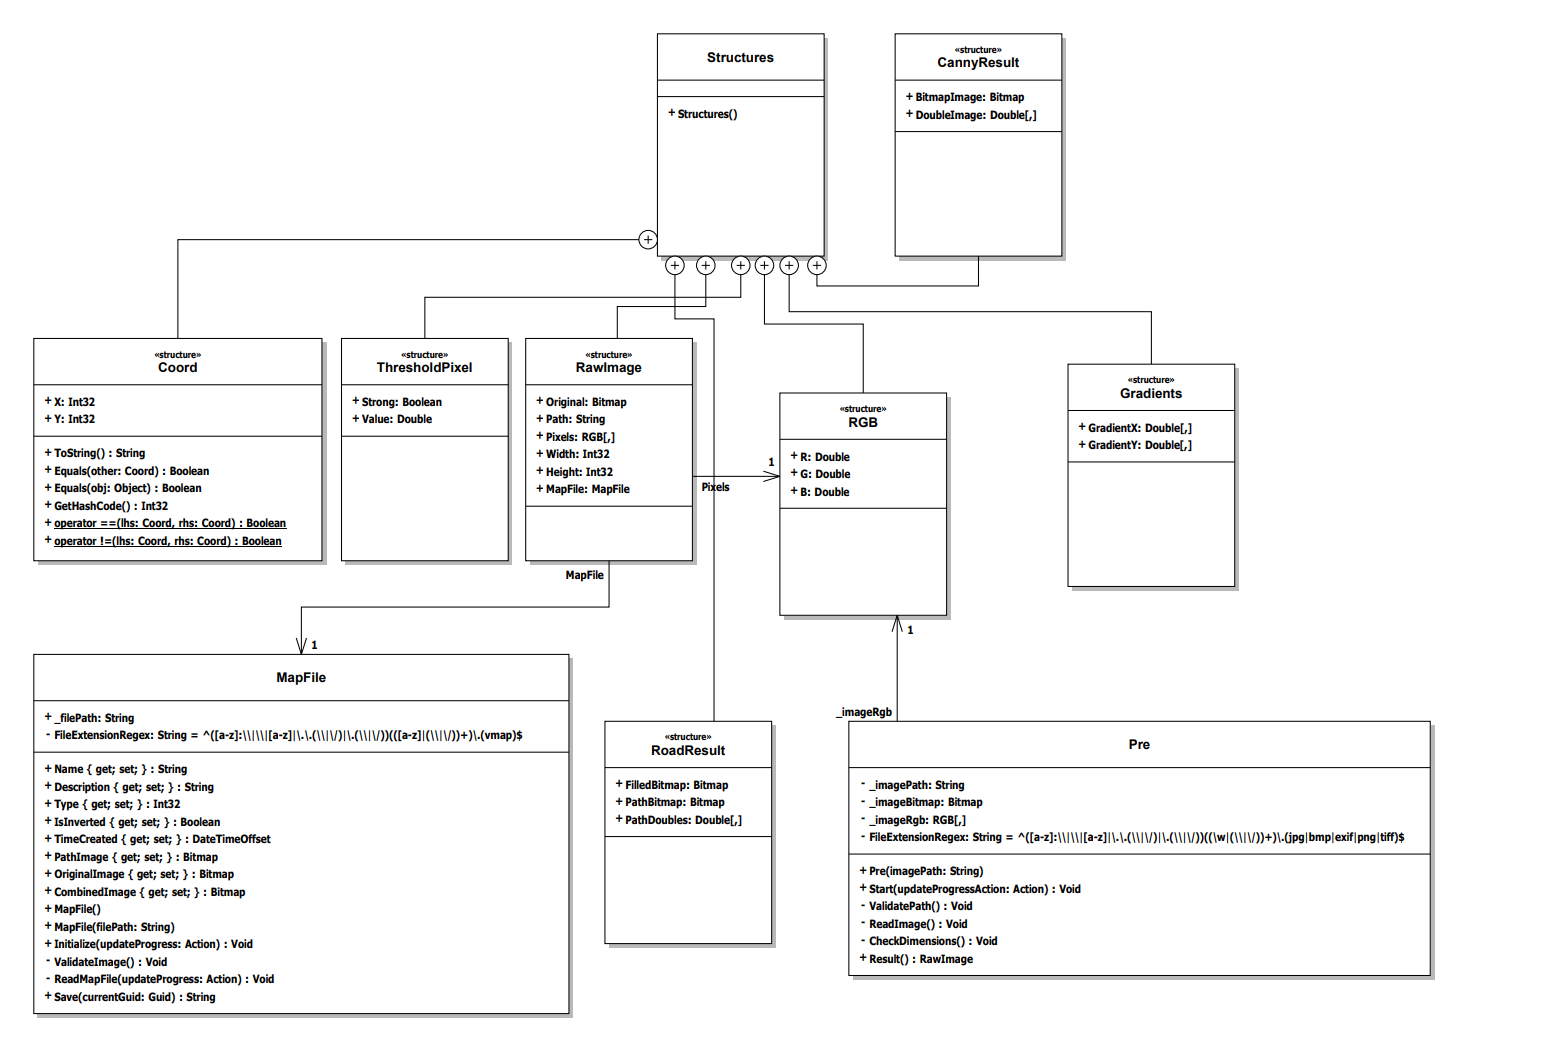
\includegraphics[width=17.2cm]{images/UML/Backend.png}}}
    \end{figure}

    \\

    As can be seen form the class diagram of the backend library, there is very little dependency within the library itself. This allows the backend to function independently of the program which is using it. This allows the backend to be split out and moved to another program if needed. Summarised there are four main reasons to do this:

    \begin{enumerate}
        \item \textbf{Modularity} - By separating the backend from the frontend one is able to be built without the other. This means that when working on my project I can take time to perfect one without impacting the other.
        \item \textbf{Reusability} - As previously stated being able to be reused is a large reason as to why to separating the elements is a good idea. Since if I wanted to expand this project for example and make a web interface for it, I could take the maths of the backend and recreate the front end in a web framework like Razor Pages.
        \item \textbf{Maintainability} - It is allot easier to maintain code when it has been organised into classes and by extension into libraries where a library is a collection of classes. It means that should something throw an error in the backend I would be able to easily isolate the issue and be able to fix it.
        \item \textbf{Testability} - In a similar vain to the Maintainability of the program being modular also means that it is very easy to implement testing. This means that as I go thorough making my program it will make it allot easier to separate variables and make isolated testing conditions. Furthermore it means that I can test the maths of the Canny Detection without having to worry about making an interface to it using the UI.
    \\ \BK

    \subsubsection{Local Application}
    The local application part of this program will be responsible for the tying if the various algorithms of the backend together along with providing the user with a way to interact with them, whether this is through the use of windows forms of the console for text inputs. As stated by objective 5 the design of the UI should be simplistic and easy to understand at a glance, therefore I will only be using the methods as stated above for interacting with the user. I also believe that it will be best to keep the changes between the two to a minimum and when there is a change make sure that the user is aware of it before hand.\\ \bk
    
    \paragraph{Design of User Interface (Console)} \mbox{} \\
    In order to keep the user interface as easy to use as possible the console will remain static while the program is being run. This means that once it has been started and set to its correct size it will form itself to fit the screen and will only run if it has been maximized. This will allow me to make sure that the interface is clear and easy to use. Find below a mock-up of the console design.
    
    \begin{figure}[H]
        \centering
        \subfloat[\centering Mock-up of Console Interface]{{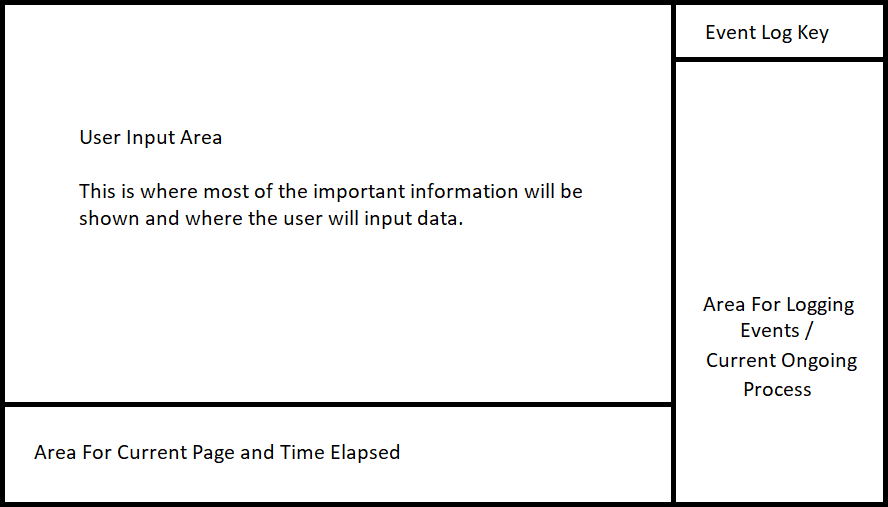
\includegraphics[width=12.5cm]{images/design/consoleMock.png}}}
    \end{figure}\\

    As can be seen in this mock-up fo the console interface it can be seen that there is a large section for the user to enter and view important in. As will be expanded on in the second section about the Windows Forms interface, due to the static nature of the console I will be able to make a Form conform to the shape of this area. See the next paragraph for more information. \\ \bk

    As for the other elements of the console UI, as part of objective 5, this must be easy to see at a glance what is going on and which step you are in. To accomplish this on the right hand side of the console there will be a log which, should the user select to do so in settings, will display each method call and the result of that call allowing them to see exactly where they are in the process. \\ \bk
    
    At the bottom of the console in the section labelled "Area for Current Page and Time Elapsed" this will be used for, as the name suggests, the current page and time elapsed. What this means is that at a glance a non-technical user or one who has opted not to have the advanced logging will still be able to see where they area at in the current process. \\ \bk

    \begin{figure}[H]
        \centering
        \subfloat[\centering Mock-up of Console Interface]{{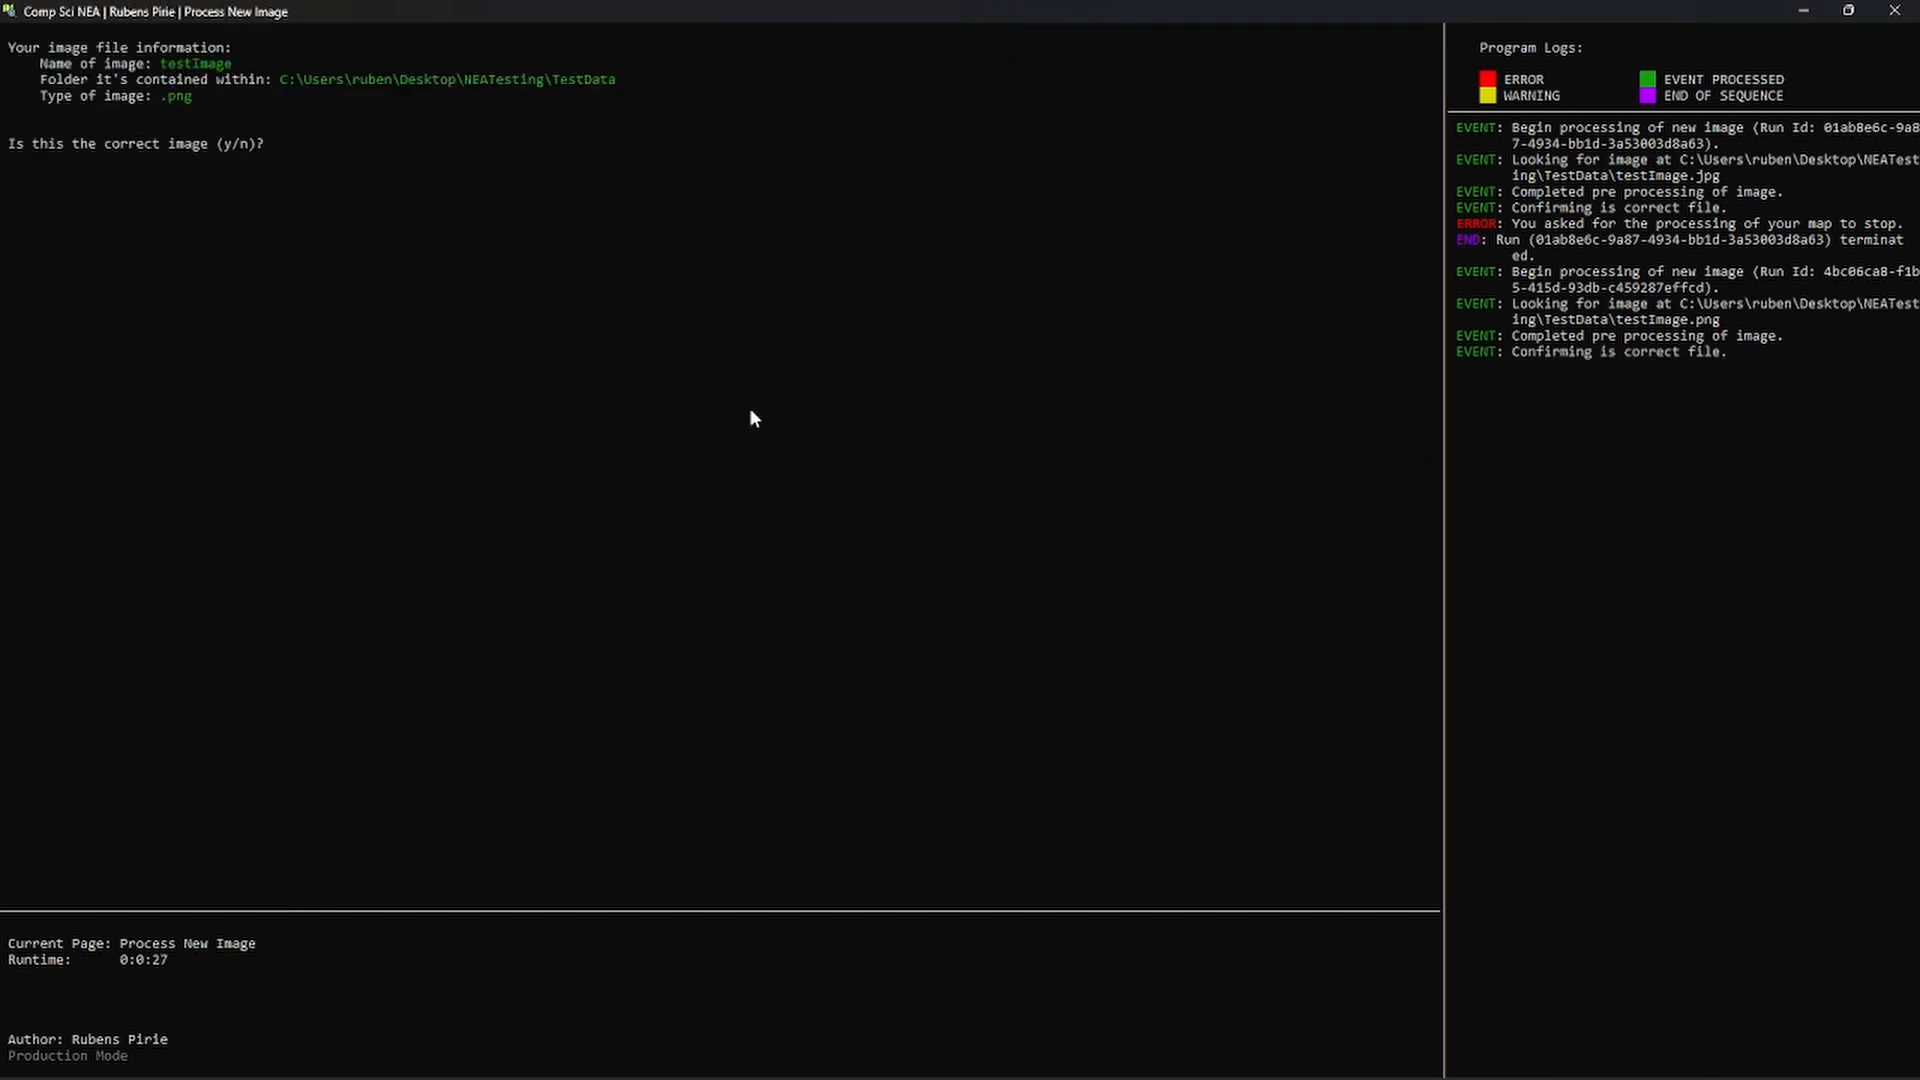
\includegraphics[width=12.5cm]{images/design/terminal.png}}}
    \end{figure}\\
    
    \BK

    \paragraph{Design of User Interface (Windows Forms)} \mbox{} \\
    For the forms interface I have chosen to keep the use of the opening of new windows to a minimum, as explained above I want this part of the program to be as simple as possible to avoid over stimulating the user and confusing them. 

    \begin{figure}[H]
        \centering
        \subfloat[\centering Windows Form For Confirming Image]{{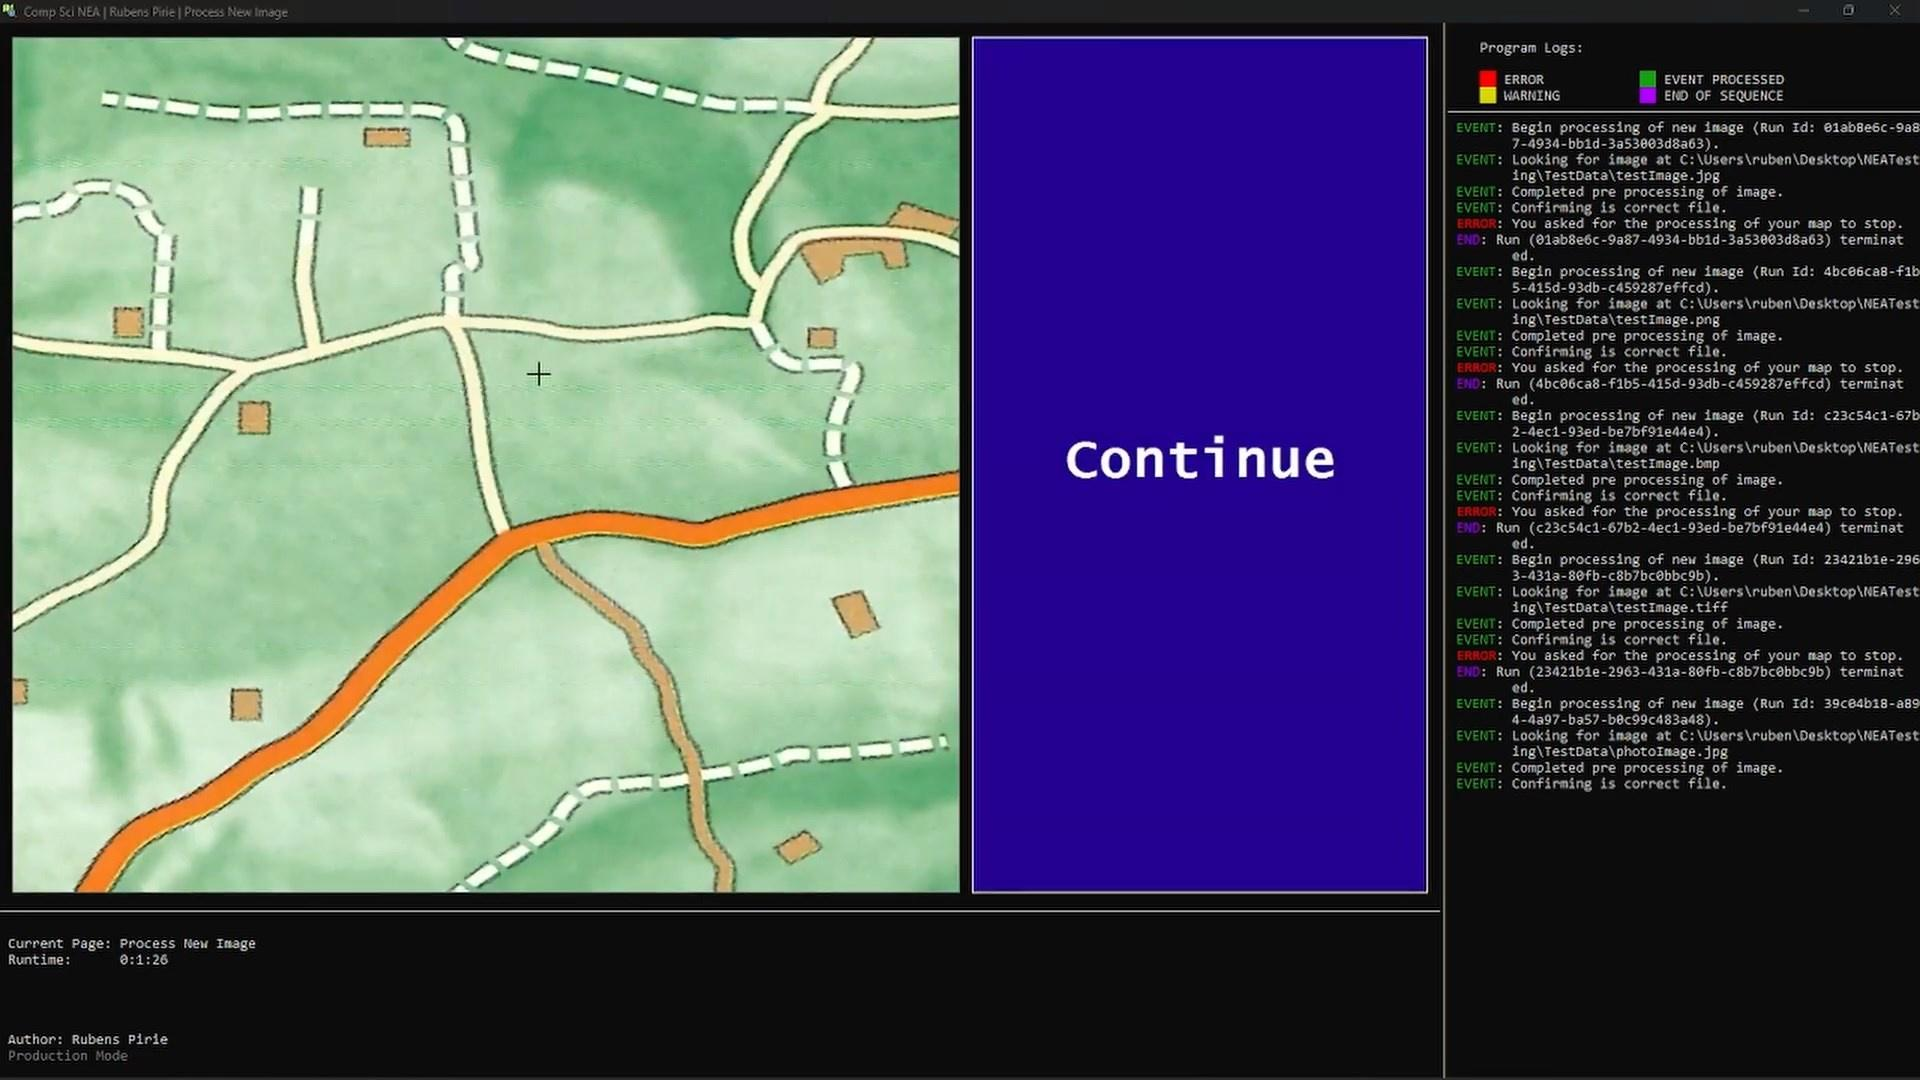
\includegraphics[width=12.5cm]{images/design/confirmWindow.jpeg}}}
    \end{figure}\\

    \begin{figure}[H]
        \centering
        \subfloat[\centering Windows Form For Pathfinding Image]{{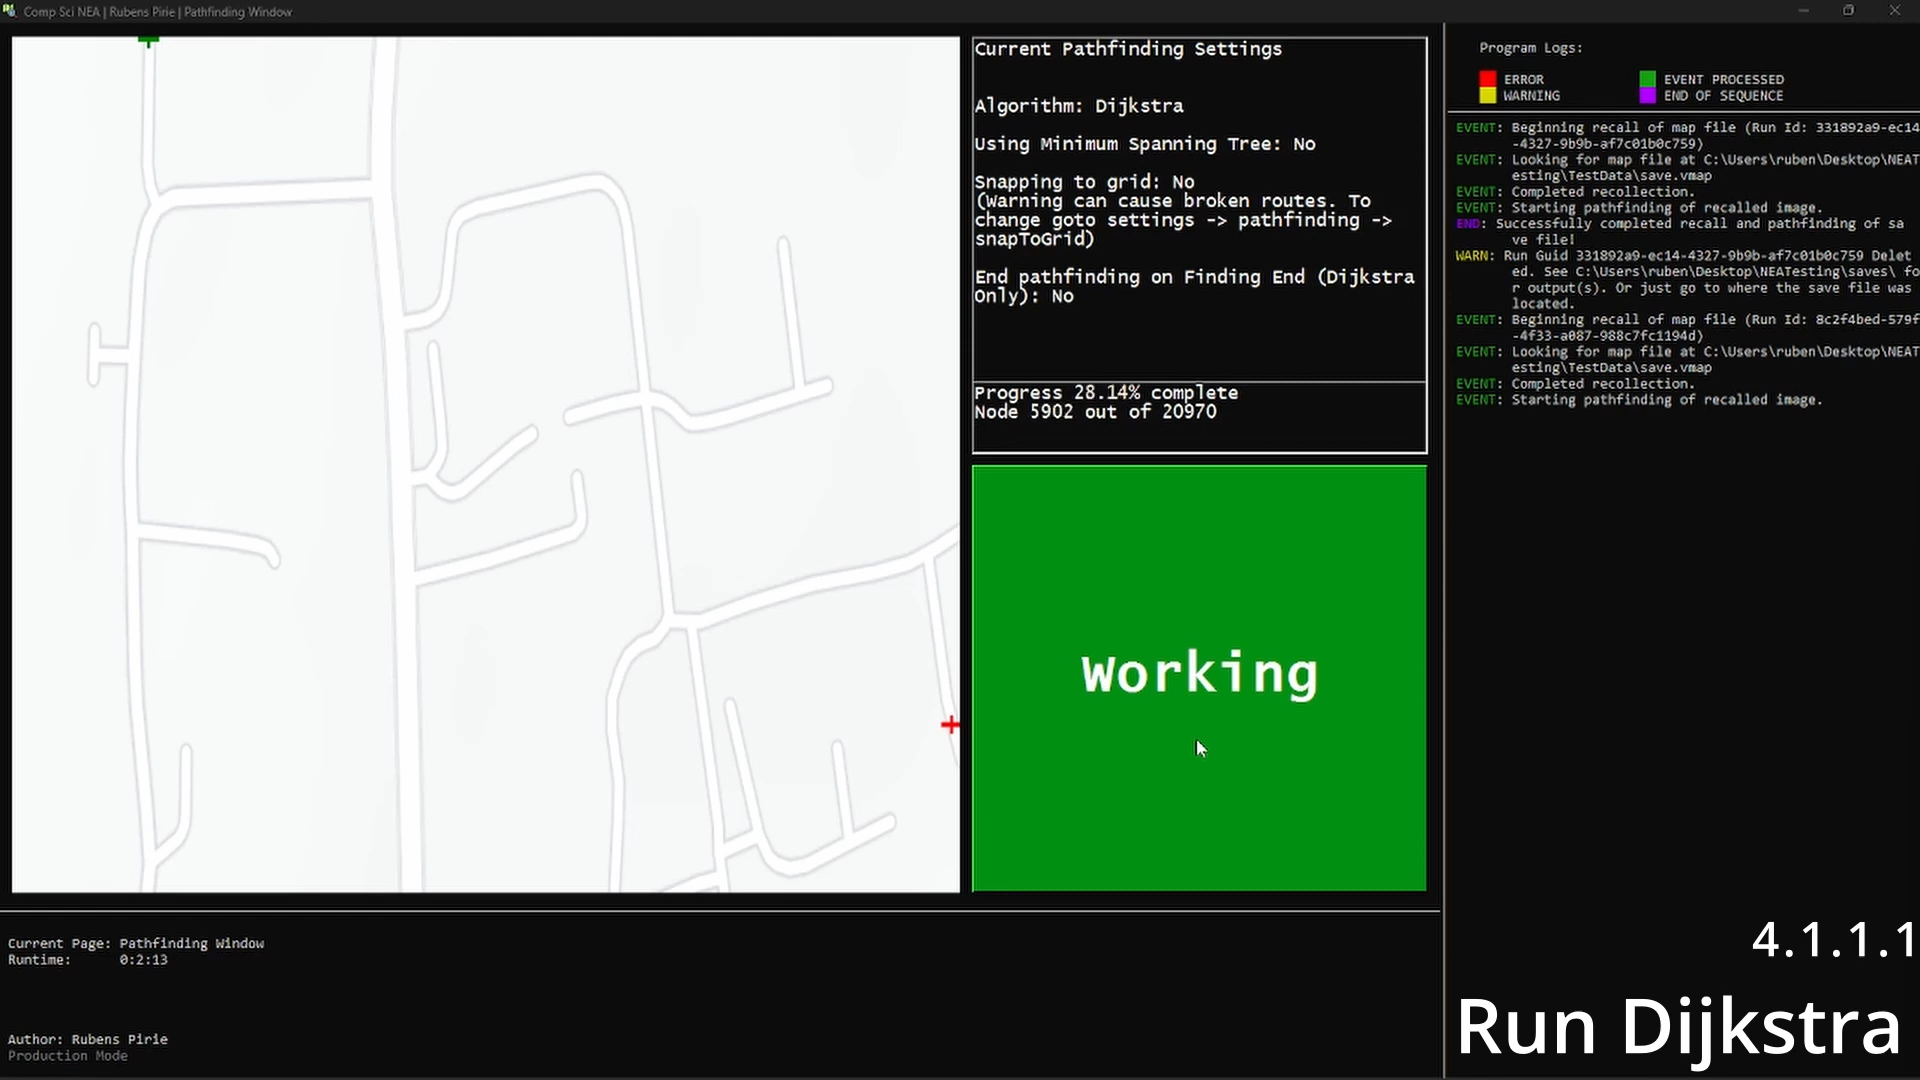
\includegraphics[width=12.5cm]{images/design/pathfindWindow.png}}}
    \end{figure}\\

    \\ \BK


    \\ \bk

    \subsection{Class Overviews}

    In this following part of the write up will go briefly over every class in the program first stating its function, which section it is in (backend library or front end application) and finally how it plays a part in the program.

    \paragraph{Canny Edge Detection \textit{(Class)}} \mbox{} \\

    \begin{figure}[H]
        \centering
        \subfloat[\centering Canny Edge Detection Class Diagram]{{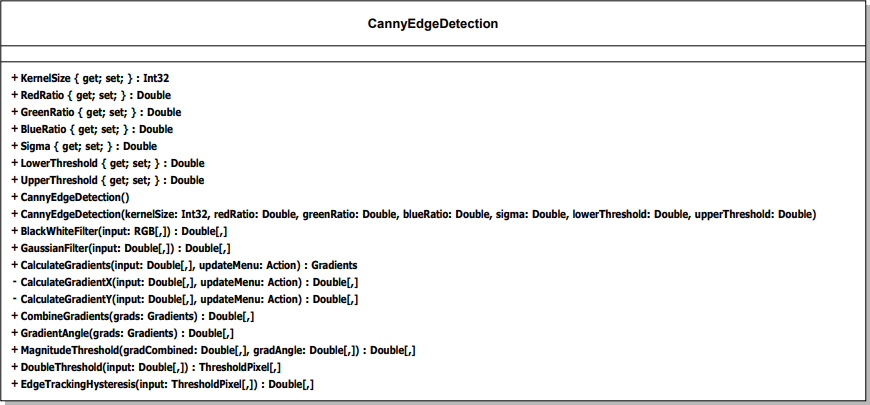
\includegraphics[width=12.5cm]{images/UML/CannyEdgeDetection.png}}}
    \end{figure}\\

    \bk


    \paragraph{Canny Result \textit{(Class)}} \mbox{} \\

    \begin{figure}[H]
        \centering
        \subfloat[\centering Canny Result Class Diagram]{{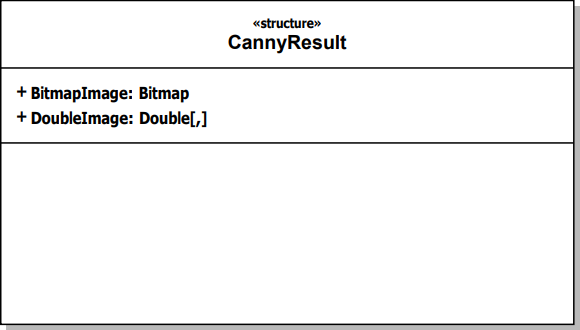
\includegraphics[width=12.5cm]{images/UML/CannyResult.png}}}
    \end{figure}\\

    \bk

    \paragraph{Coord \textit{(Structure)}} \mbox{} \\

    \begin{figure}[H]
        \centering
        \subfloat[\centering Coord Class Diagram]{{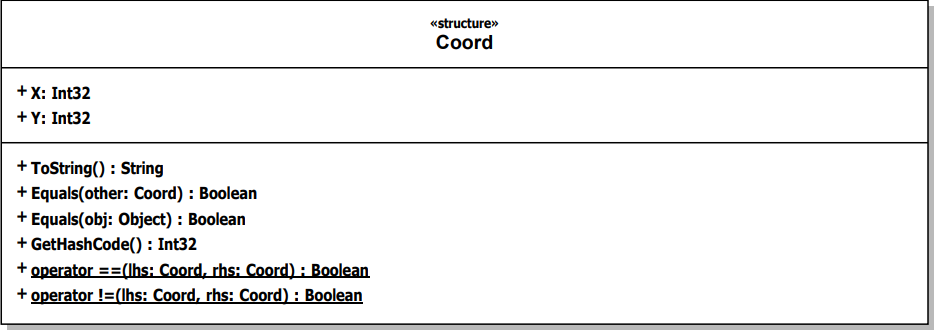
\includegraphics[width=12.5cm]{images/UML/Coord.png}}}
    \end{figure}\\

    \bk

    \paragraph{Extensions \textit{(Class)}} \mbox{} \\

    \begin{figure}[H]
        \centering
        \subfloat[\centering Extensions Class Diagram]{{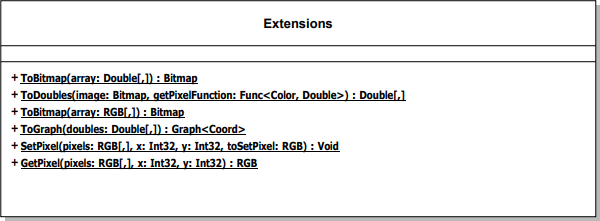
\includegraphics[width=12.5cm]{images/UML/Extensions.png}}}
    \end{figure}\\

    \bk

    \paragraph{Gradients \textit{(Structure)}} \mbox{} \\

    \begin{figure}[H]
        \centering
        \subfloat[\centering Gradients Class Diagram]{{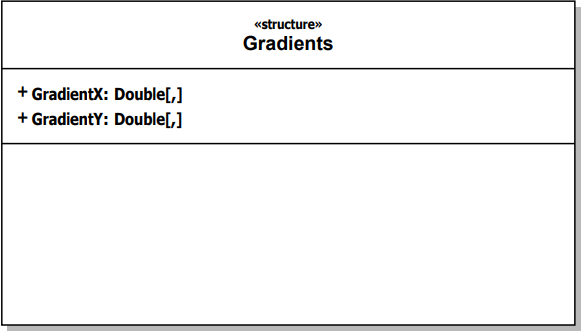
\includegraphics[width=12.5cm]{images/UML/Gradients.png}}}
    \end{figure}\\

    \bk


    \paragraph{Graph \textit{(Class)}} \mbox{} \\

    \begin{figure}[H]
        \centering
        \subfloat[\centering Graph Class Diagram]{{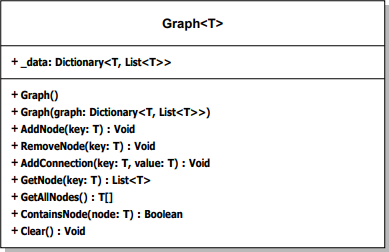
\includegraphics[width=12.5cm]{images/UML/Graph.png}}}
    \end{figure}\\

    \bk

    \paragraph{Graph Exception \textit{(Exception)}} \mbox{} \\

    \begin{figure}[H]
        \centering
        \subfloat[\centering Graph Exception Class Diagram]{{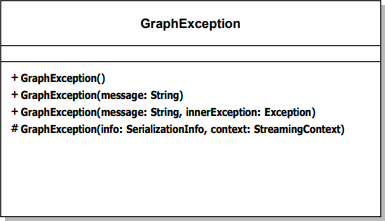
\includegraphics[width=12.5cm]{images/UML/GraphException.png}}}
    \end{figure}\\

    \bk

    \paragraph{IHandler \textit{(Interface)}} \mbox{} \\

    \begin{figure}[H]
        \centering
        \subfloat[\centering IHandler UML Diagram]{{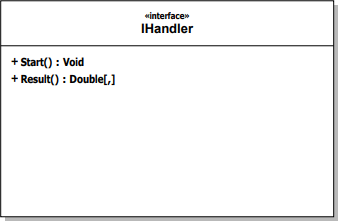
\includegraphics[width=12.5cm]{images/UML/IHandler.png  }}}
    \end{figure}\\

    \bk

    
    \paragraph{Input \textit{(Class)}} \mbox{} \\

    \begin{figure}[H]
        \centering
        \subfloat[\centering Input Class Diagram]{{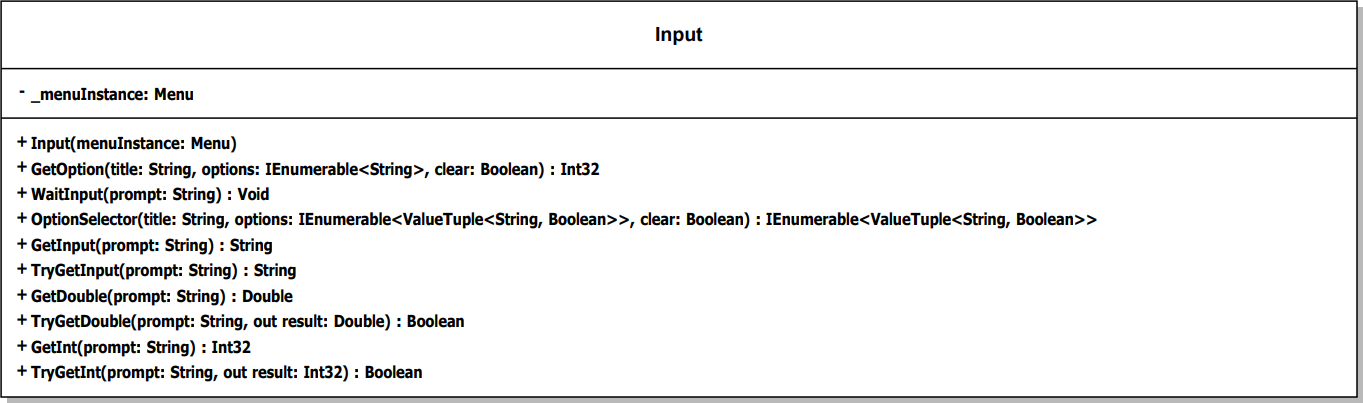
\includegraphics[width=12.5cm]{images/UML/Input.png}}}
    \end{figure}\\

    \bk

    
    \paragraph{Kernel \textit{(Class)}} \mbox{} \\

    \begin{figure}[H]
        \centering
        \subfloat[\centering Kernel Class Diagram]{{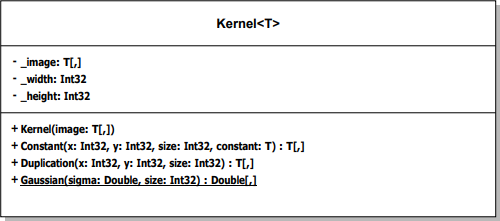
\includegraphics[width=12.5cm]{images/UML/Kernel.png}}}
    \end{figure}\\

    \bk

    
    \paragraph{Kernel Exception \textit{(Exception)}} \mbox{} \\

    \begin{figure}[H]
        \centering
        \subfloat[\centering Kernel Exception Class Diagram]{{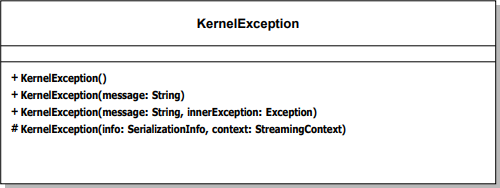
\includegraphics[width=12.5cm]{images/UML/KernelException.png}}}
    \end{figure}\\

    \bk

    \paragraph{Logger \textit{(Class)}} \mbox{} \\

    \begin{figure}[H]
        \centering
        \subfloat[\centering Logger Class Diagram]{{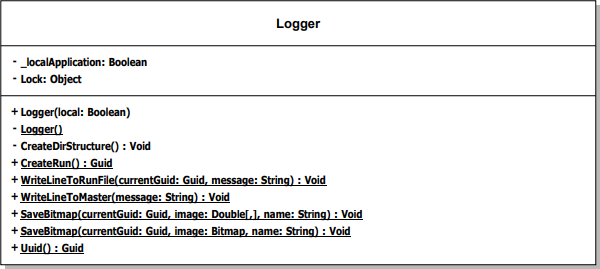
\includegraphics[width=12.5cm]{images/UML/Logger.png}}}
    \end{figure}\\

    \bk

    \paragraph{Logger Exception \textit{(Exception)}} \mbox{} \\

    \begin{figure}[H]
        \centering
        \subfloat[\centering Logger Exception Class Diagram]{{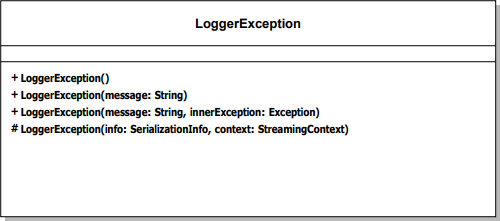
\includegraphics[width=12.5cm]{images/UML/LoggerException.png}}}
    \end{figure}\\

    \bk

    \paragraph{Map File Exception \textit{(Exception)}} \mbox{} \\

    \begin{figure}[H]
        \centering
        \subfloat[\centering Map File Exception Class Diagram]{{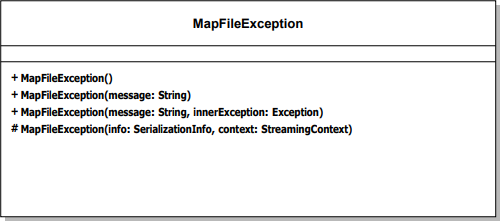
\includegraphics[width=12.5cm]{images/UML/MapFileException.png}}}
    \end{figure}\\

    \bk

    \paragraph{Matrix \textit{(Class)}} \mbox{} \\

    \begin{figure}[H]
        \centering
        \subfloat[\centering Matrix Class Diagram]{{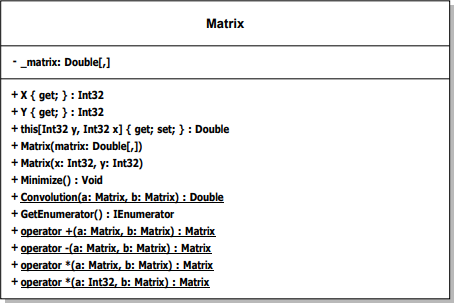
\includegraphics[width=12.5cm]{images/UML/Matrix.png}}}
    \end{figure}\\

    \bk

    \paragraph{Matrix Exception \textit{(Exception)}} \mbox{} \\

    \begin{figure}[H]
        \centering
        \subfloat[\centering Matrix Exception Class Diagram]{{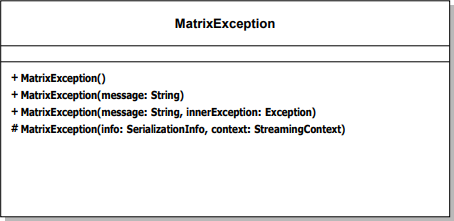
\includegraphics[width=12.5cm]{images/UML/MatrixException.png}}}
    \end{figure}\\

    \bk


    \paragraph{Max Priority Queue \textit{(Class)}} \mbox{} \\

    \begin{figure}[H]
        \centering
        \subfloat[\centering Max Priority Queue Class Diagram]{{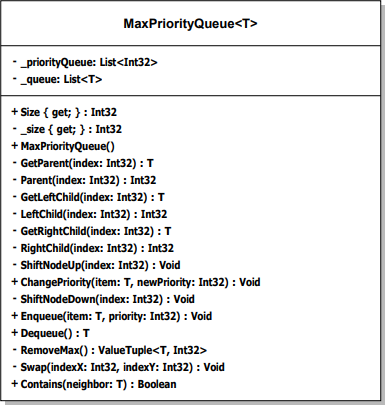
\includegraphics[width=12.5cm]{images/UML/MaxPriorityQueue.png}}}
    \end{figure}\\

    \bk

    
    \paragraph{Min Priority Queue \textit{(Class)}} \mbox{} \\

    \begin{figure}[H]
        \centering
        \subfloat[\centering Min Priority Queue Class Diagram]{{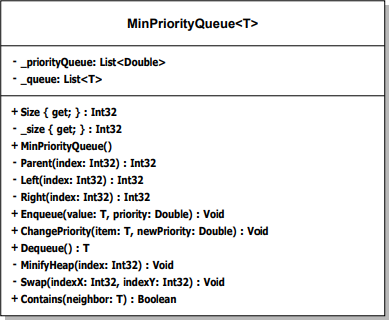
\includegraphics[width=12.5cm]{images/UML/MinPriorityQueue.png}}}
    \end{figure}\\

    \bk

    \paragraph{Pathfinder \textit{(Class)}} \mbox{} \\

    \begin{figure}[H]
        \centering
        \subfloat[\centering Pathfinder Class Diagram]{{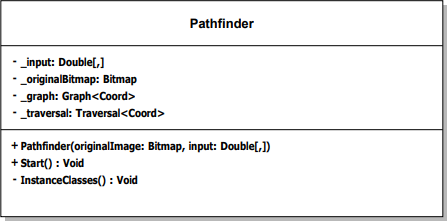
\includegraphics[width=12.5cm]{images/UML/Pathfinder.png}}}
    \end{figure}\\

    \bk

    \paragraph{Pathfind Image Form \textit{(Windows Form)}} \mbox{} \\

    \begin{figure}[H]
        \centering
        \subfloat[\centering Pathfind Image Form UML Diagram]{{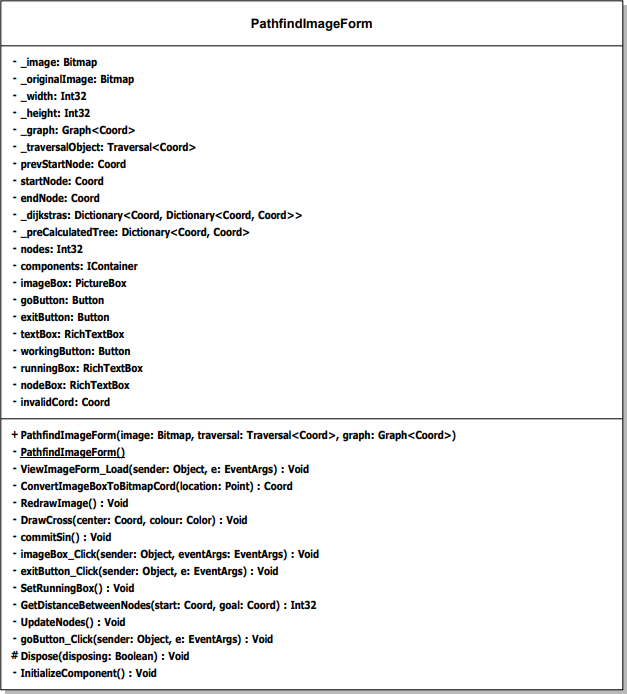
\includegraphics[width=12.5cm]{images/UML/PathfindImageForm.png}}}
    \end{figure}\\

    \bk

    \paragraph{Post \textit{(Class)}} \mbox{} \\

    \begin{figure}[H]
        \centering
        \subfloat[\centering Post Class Diagram]{{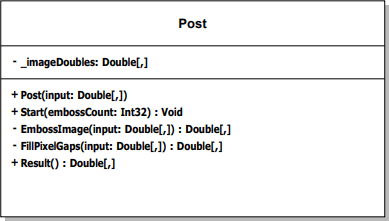
\includegraphics[width=12.5cm]{images/UML/Post.png}}}
    \end{figure}\\

    \bk

    \paragraph{Preprocessing Exception \textit{(Exception)}} \mbox{} \\

    \begin{figure}[H]
        \centering
        \subfloat[\centering Preprocessing Exception Class Diagram]{{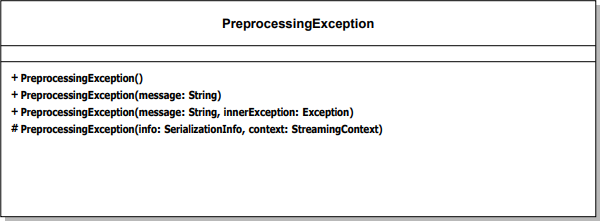
\includegraphics[width=12.5cm]{images/UML/PreprocessingException.png}}}
    \end{figure}\\

    \bk

    \paragraph{Program \textit{(Class)}} \mbox{} \\

    \begin{figure}[H]
        \centering
        \subfloat[\centering Program Class Diagram]{{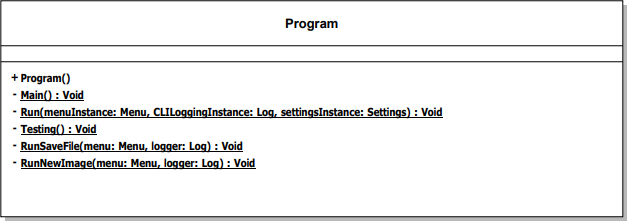
\includegraphics[width=12.5cm]{images/UML/Program.png}}}
    \end{figure}\\

    \bk

    \paragraph{Queue \textit{(Class)}} \mbox{} \\

    \begin{figure}[H]
        \centering
        \subfloat[\centering Queue Class Diagram]{{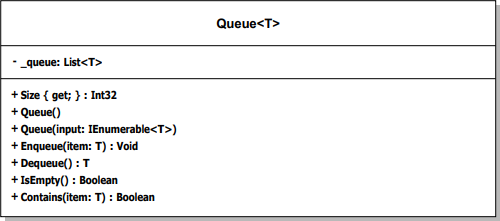
\includegraphics[width=12.5cm]{images/UML/Queue.png}}}
    \end{figure}\\

    \bk

    \paragraph{Road Detection \textit{(Class)}} \mbox{} \\

    \begin{figure}[H]
        \centering
        \subfloat[\centering Road Detection Class Diagram]{{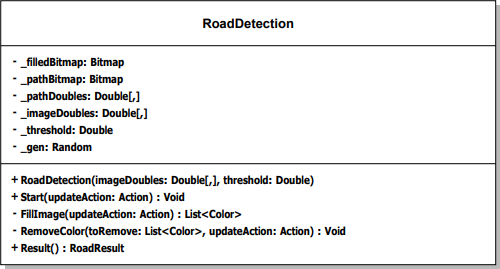
\includegraphics[width=12.5cm]{images/UML/RoadDetection.png}}}
    \end{figure}\\

    \bk

    \paragraph{Settings Exception \textit{(Exception)}} \mbox{} \\

    \begin{figure}[H]
        \centering
        \subfloat[\centering Settings Exception Class Diagram]{{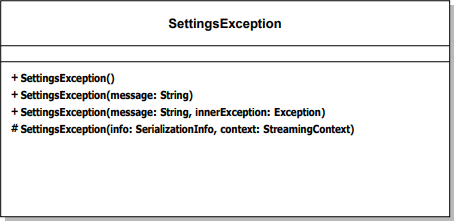
\includegraphics[width=12.5cm]{images/UML/SettingsException.png}}}
    \end{figure}\\

    \bk

    \paragraph{Stack \textit{(Class)}} \mbox{} \\

    \begin{figure}[H]
        \centering
        \subfloat[\centering Stack Class Diagram]{{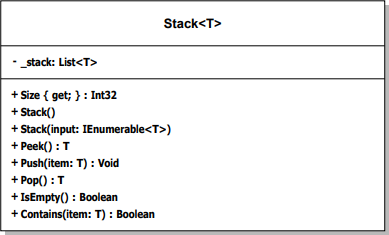
\includegraphics[width=12.5cm]{images/UML/Stack.png}}}
    \end{figure}\\

    \bk

    \paragraph{Text Wall \textit{(Class)}} \mbox{} \\

    \begin{figure}[H]
        \centering
        \subfloat[\centering Text Wall Class Diagram]{{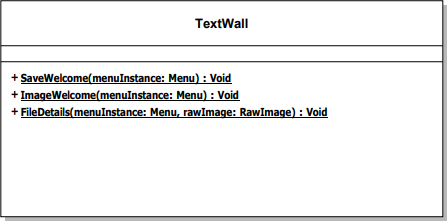
\includegraphics[width=12.5cm]{images/UML/TextWall.png}}}
    \end{figure}\\

    \bk

    \paragraph{Traversal \textit{(Class)}} \mbox{} \\

    \begin{figure}[H]
        \centering
        \subfloat[\centering Traversal Class Diagram]{{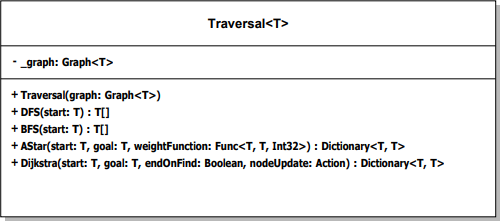
\includegraphics[width=12.5cm]{images/UML/Traversal.png}}}
    \end{figure}\\

    \bk

    \paragraph{Utility \textit{(Class)}} \mbox{} \\

    \begin{figure}[H]
        \centering
        \subfloat[\centering Utility Class Diagram]{{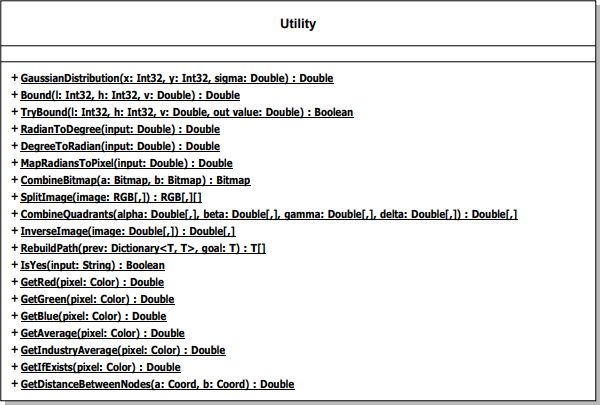
\includegraphics[width=12.5cm]{images/UML/Utility.png}}}
    \end{figure}\\

    \bk

    \paragraph{View Image Form \textit{(Windows Form)}} \mbox{} \\

    \begin{figure}[H]
        \centering
        \subfloat[\centering View Image Form UML Diagram]{{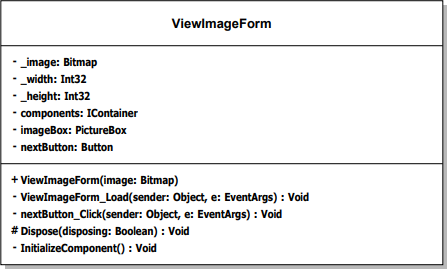
\includegraphics[width=12.5cm]{images/UML/ViewImageForm.png}}}
    \end{figure}\\

    \bk

    








\end{flushleft}